\documentclass[10pt,a4paper]{article}
\usepackage[utf8]{inputenc}
\usepackage{amsmath}
\usepackage{amsfonts}
\usepackage{amssymb}
\usepackage{amsthm}
\usepackage{enumerate}
\usepackage{graphicx}
\usepackage{appendix}
\newtheorem{proposition}{Proposition}
\newtheorem{lemma}{Lemma}
\newtheorem{theorem}{Theorem}
\newtheorem{definition}{Definition}
\theoremstyle{remark}
\newtheorem{example}{Example}
\newtheorem{exercise}{Exercise}
\newtheorem{remark}{Remark}
\usepackage[left=2cm,right=2cm,top=2cm,bottom=2cm]{geometry}

\author{Hao Peng}
\title{Condition-based Maintenance}
\begin{document}
\maketitle
\section{Introduction}
According to the classification of maintenance strategies in \cite{Arts14}, condition-based maintenance (CBM) is one type of preventive maintenance policy. CBM has attracted lots of attentions of both academia and industry due to the development of advanced sensor technology and measurement equipments. The major difference of CBM compared with other maintenance strategies is the utilization of the advanced information about the health status of a component or a system. Let us first remind ourselves about what kind of information we used to get an age-based policy or block replacement policy.

For age-based policy or block replacement policy, the information needed is the failure time distributions of components or systems. For example, in the calculation of age-based policy, we need to know the distribution function of the random lifetime of a component, $F_{T}(\cdot)$. In the calculation of block replacement policy, we need to know the expected number of failures during an interval, $M_{T}(\tau)$, which is also derived based on the failure time distribution. By using the failure time distribution to describe the health status of a component or a system, we assume there are two states for a component or a system, i.e., the failure state and the working state. The random failure time $T$ is the duration of the working state.

For condition-based policies, systems or components have multiple intermediate states in between the failure state and the perfect/newest state. The transition of degradation states can be described by many different types of probability models, e.g., Delay Time model, Markov process. Or, the deterioration of systems may follow a continuous stochastic process, e.g., random coefficient model, gamma process, Wiener process. Then the system state is continuous. Based on the information of degradation processes, the inspection and replacement decisions can be made to optimize the CBM policies. Renewal theory may be used to evaluate the expected total cost rate. Markov decision process is also an analytical tool to formulate the problem. In this chapter, we mainly demonstrate the evaluation of average total cost rate by renewal theory for single-component systems. 

\section{Delay Time Model}
The Delay Time Model (DTM) was first developed by \cite{ChristerWaller84}. It assumes that a component or a system has three states: normal, defective and failed. 
\begin{figure}[h!!!]  % ��ͼ���� i
  % Requires \usepackage{graphicx}
  \centering
  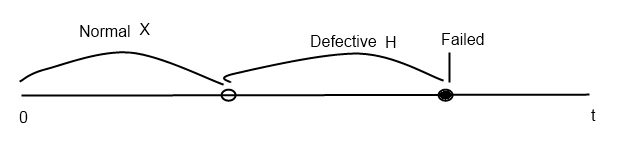
\includegraphics[width=6in]{DTM1.png}\\
  \footnotesize
  \caption{ \footnotesize{ The Delay Time Model} }\label{DTM1}
\end{figure}

As shown in Figure \ref{DTM1}, the duration of the normal state, also referred to as the time to defect, is a continuous non-negative random variable denoted by $X$. The duration of the defective state, also referred to as the delay time, is a continuous non-negative random variable denoted by $H$. The cumulative distribution function and the probability density function of the time to defect are denoted by $F_{X}(\cdot)$ and $f_{X}(\cdot)$ respectively. The cumulative distribution function and the probability density function of the delay time are denoted by $F_{H}(\cdot)$ and $f_{H}(\cdot)$ respectively. 

Under the normal state, the system works fine and defects do not exist in the system. Under the defective state, the system still works but the defects of the system appear and can only be detected by inspections. The failure state of the system is self-announcing. The advanced information considered by DTM as we can tell is the defective information obtained through inspections, compared with the age-based policy or block replacement policy. Given such information, we are interested in obtaining the optimal inspection and maintenance policy.

The DTM is an abstract of many engineering systems. Of course, it is a simplified description of complex failure mechanisms. But for most of the cases (see example \ref{ex:DTM}), this simplification works pretty well for maintenance optimization.
\begin{example} \label{ex:DTM} \renewcommand{\qedsymbol}{$\lozenge$} \mbox{}
\begin{enumerate}
\item The condition of ball-bearings can be measured via the amplitude of vibrations around the bearing. After a certain period of operating, the condition of ball-bearings becomes less good and the amplitude of vibrations becomes larger. The engineers define a certain limit of vibration above which the engineers will see the system as ""defective". The system will stay in the defective state for a while till breakdown.
\item The condition of a metal part can be determined by visually inspecting the number and length of cracks. After a certain period of operating, the condition of a metal part becomes worse. The engineers define a certain criteria for cracks to determine the system state as "defective". The system will stay in the defective state for a while till breakdown.
\item For metal systems with moving parts, the concentration of ferrous parts in the lubrication fluid is measured as an indication of the wear. After a certain period of operating, the concentration of ferrous parts becomes larger. The engineers define a certain limit for this concentration measurement above which the system is seen as "defective". The system will stay in this defective state for a while till breakdown.
\end{enumerate}
\qed
\end{example}

\subsection{A periodic inspection policy for a single-component system} \label{sec:DTMmodel1} 
We consider a periodic inspection policy for a single-component system that has a single failure mode (i.e., the component is subject to one dominant failure mechanism). We inspect the system with a fixed interval $\tau$. We assume the inspections are perfect, i.e., if the system is in the defective state the inspections can detect it immediately. Our maintenance policy is that if we detect the defective state upon inspections, we will immediately replace the component with a new one. If the component fails before the next scheduled inspection takes place, we will perform a breakdown corrective maintenance action immediately. The maintenance time is negligible. Notice that there are two types of renewal events in this periodic inspection policy, i.e., the inspection renewal when defects are found and the breakdown renewal. After the system is renewed by a new component, the inspections are rescheduled from the renewal point.

We assume the inspection cost is $C_{i}$. The preventive maintenance cost is $C_{pm}$, which is the replacement cost. The corrective maintenance cost is $C_{cm}$, which is the replacement cost plus the failure cost. 

We first consider a simple case that the time to defect $X$ follows an exponential distribution. According to the memory less property of the exponential distribution, this implies an inspection renews the system regardless whether a defect was identified or not. Since each failure or inspection renews the system with associated costs, the process is a renewal reward process, and the long term expected cost per unit time, $CR(\tau)$, is given by, 
\begin{align} \label{eq:renew}
CR(\tau)=\lim_{t \to \infty}\dfrac{C(t)}{t}=\dfrac{E[CC]}{E[CL]},
\end{align}
where $C(t)$ is the expected total cost till time $t$, $E[CC]$ is the expected renewal cycle cost and $E[CL]$ is the expected renewal cycle length which is the interval between two consecutive renewals. 

Let us first look at the expected renewal cycle length. Starting with a renewal point, if the failure time $X+H$ is larger than the inspection interval $\tau$, then the system gets renewed at time point $\tau$, i.e., the renewal cycle length is $\tau$. If the failure time $X+H$ is smaller than the inspection interval $\tau$, then the system gets renewed at a failure, which is random.

The distribution of $X+H$ is the summation of two independent random variables, which can be calculated through convolution as follows.
\begin{equation*}
f_{X+H}(t)=\int_{0}^{t}f_{X}(u)f_{H}(t-u)du,
\end{equation*}
\begin{equation*}
F_{X+H}(t)=\int_{0}^{t}f_{X}(u)F_{H}(t-u)du,
\end{equation*}
where $f_{X+H}(\cdot)$ and $F_{X+H}(\cdot)$ is the probability density function and cumulative distribution function of $X+H$ respectively.

Then the calculation of the expected renewal cycle length is very similar to how we evaluate the expected renewal cycle length for the age-based policy.
\begin{align} \label{eq:cycle length}
E[CL] & =  \int_{0}^{\tau}t f_{X+H}(t)dt + \tau (1-F_{X+H}(\tau))\nonumber \\
& = \int_{0}^{\tau}t \int_{0}^{t}f_{X}(u)f_{H}(t-u)dudt + \tau (1- \int_{0}^{\tau}f_{X}(u)F_{H}(\tau-u)du).  
\end{align}

For the expected renewal cycle cost, there are three different random events at the end of a renewal cycle to analyze, i.e., a failure, an inspection with replacement due to the defects, and an inspection without replacement. The probability of a failure renewal is the probability that the failure time $X+H$ is before the next inspection comes, i.e.,
\begin{equation*}
Pr(X+H<\tau)=F_{X+H}(\tau).
\end{equation*}
Since the failure renewal will incur a corrective maintenance cost $C_{cm}$, the expected corrective maintenance cost is $C_{cm}Pr(X+H<\tau)$. 
The probability of an inspection renewal without replacement is the probability that the time to defect $X$ is larger than the next inspection time, i.e.,
\begin{equation*}
Pr(X>\tau)=1-F_{X}(\tau).
\end{equation*}
Since this inspection renewal will only incur an inspection cost $C_{i}$, the expected cost related to the inspection renewal without replacement is $C_{i}Pr(X>\tau)$.
The probability of an inspection renewal with replacement is the probability that the time to defect $X$ is smaller than the next inspection time and the failure time $X+H$ is larger than the next inspection time, i.e.,
\begin{align*}
Pr(X<\tau \cap X+H>\tau) & = \int_{0}^{\tau} f_{X}(u) Pr(u+H>\tau)du \nonumber \\  
& = \int_{0}^{\tau} f_{X}(u) (1-F_{H}(\tau-u))du. \nonumber 
\end{align*}
Since this inspection renewal will incur an inspection cost plus the preventive maintenance cost $C_{i}+C_{pm}$, the expected cost related to the inspection renewal with replacement is $(C_{i}+C_{pm})Pr(X<\tau \cap X+H>\tau)$.
Therefore, the summation of these cost elements is the expected renewal cycle cost, i.e.,
\begin{align}\label{eq:cycle cost} 
E[CC]=C_{cm}Pr(X+H<\tau)+C_{i}Pr(X>\tau)+(C_{i}+C_{pm})Pr(X<\tau \cap X+H>\tau). 
\end{align} 
Notice that the summation of the probabilities of the three renewal events is one. After calculating the expected renewal cycle length and the expected renewal cycle cost using Equation \ref{eq:cycle length} and \ref{eq:cycle cost}, we can obtain the average long run cost rate by Equation \ref{eq:renew}. 
\begin{example} \label{ex:DTM1} \renewcommand{\qedsymbol}{$\lozenge$} \mbox{} 

Assume both the time to defect and the delay time distributions are exponential with parameters $\lambda_{X}$ 0.6 and $\lambda_{H}$ 0.75 respectively ($f(t)=\lambda exp (-\lambda t)$). The time unit is 100 days and the cost parameter values are $C_{cm}=1000$, $C_{pm}=150$, and $C_{i}=15$ respectively. Using Equation \ref{eq:renew}, \ref{eq:cycle length} and \ref{eq:cycle cost}, the expected long run cost per unit time as a function of $\tau$ is shown in Figure \ref{pic:example1}.

The distribution of $X+H$ is the summation of two independent exponential random variables, which can be calculated through convolution as follows.
\begin{align}
f_{X+H}(t) & =\int_{0}^{t}f_{X}(u)f_{H}(t-u)du \nonumber \\
& = \lambda_{X} \lambda_{H} \int_{0}^{t} exp(-\lambda_{X} u) exp(-\lambda_{H} (t-u)) du \nonumber \\
& = \lambda_{X} \lambda_{H} exp(-\lambda_{H} t) \int_{0}^{t} exp(-\lambda_{X} u+\lambda_{H}u) du \nonumber \\
& = \dfrac{\lambda_{X} \lambda_{H}}{\lambda_{H}-\lambda_{X}}(exp(-\lambda_{X} t)-exp(-\lambda_{H}t)). 
\end{align}
\begin{align}
F_{X+H}(t) & =\int_{0}^{t}f_{X}(u)F_{H}(t-u)du \nonumber \\
& =  \lambda_{X}\int_{0}^{t} exp(-\lambda_{X}u) (1-exp(-\lambda_{H}(t-u))) du \nonumber \\
& = 1+\dfrac{-\lambda_{H}exp(-\lambda_{X}t+\lambda_{X}exp(-\lambda_{H}t))}{-\lambda_{X}+\lambda_{H}}
\end{align}

Then the expected renewal cycle length can be obtained by Equation \ref{eq:cycle length}.

\begin{align}
Pr(X<\tau \cap X+H>\tau) & = \int_{0}^{\tau} f_{X}(u) Pr(u+H>\tau)du \nonumber \\  
& = \int_{0}^{\tau} f_{X}(u) (1-F_{H}(\tau-u))du \nonumber \\
& = \lambda_{X}\int_{0}^{\tau} exp(-\lambda_{X}u) exp(-\lambda_{H}(\tau-u)) du \nonumber \\
& = \dfrac{\lambda_{X}}{-\lambda_{X}+\lambda_{H}}(exp(-\lambda_{X}\tau)-exp(-\lambda_{H}\tau))
\end{align}

Then the expected renewal cycle cost can be obtained by Equation \ref{eq:cycle cost}.

\begin{figure}[h!!!]  % ��ͼ���� i
  % Requires \usepackage{graphicx}
  \centering
  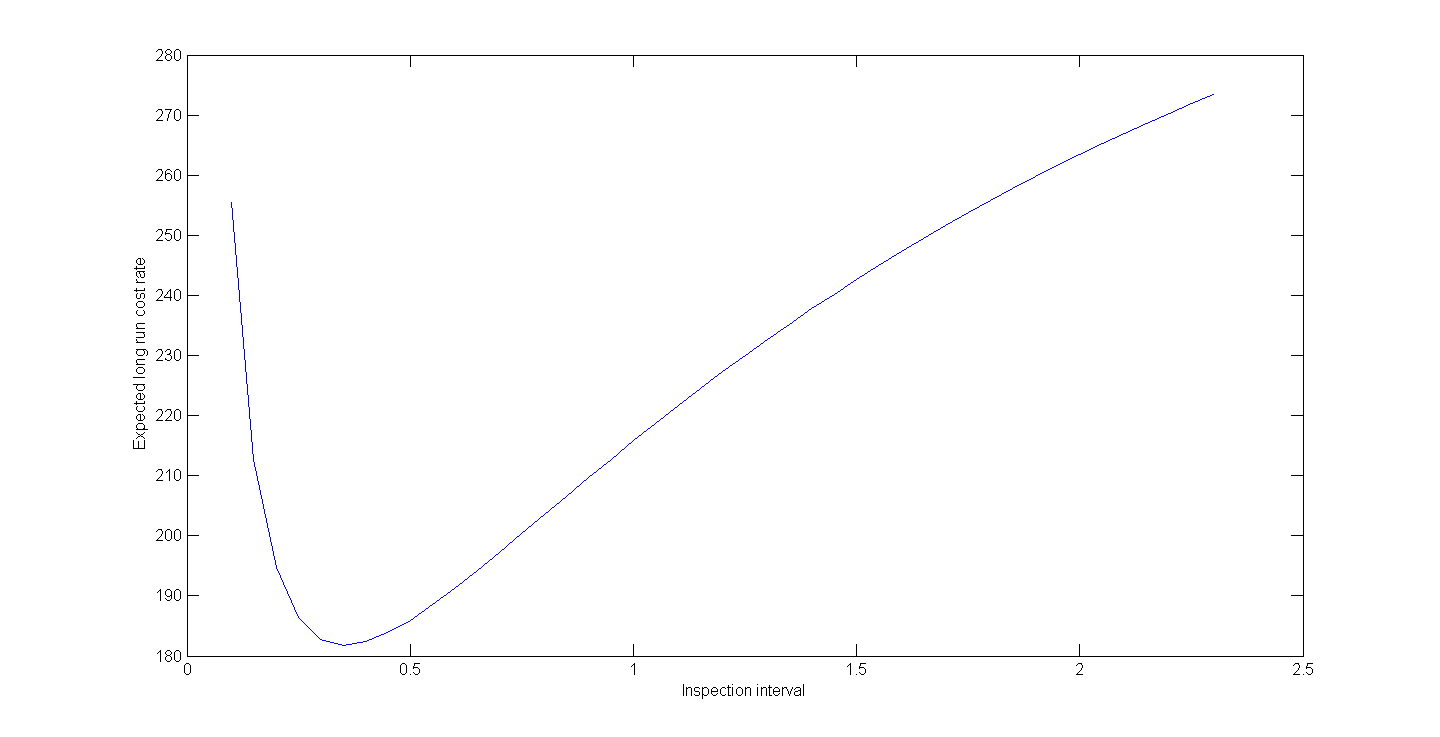
\includegraphics[width=6in]{example1.png}\\
  \footnotesize
  \caption{ \footnotesize{Expected cost per unit time v inspection interval} }\label{pic:example1}
\end{figure}

The optimal inspection interval is $0.4 \times 100=40$ days. 
\qed
\end{example}

\subsection{A generalized periodic inspection policy for a single-component system}

If the time to defect $X$ does not follow an exponential distribution, not all the inspection time points are the renewal points as we discussed in Section \ref{sec:DTMmodel1}. 

In this case a renewal cycle may span several inspection intervals. Following the same analysis procedure of renewal theory, we distinguish two renewal events, i.e., the failure renewal and the inspection renewal with replacement. Again, we are interested in the probabilities of the two renewal events. The probability that the failure renewal occurs in a certain inspection interval $((i-1)\tau,i\tau)$ is the probability that the failure happens in the inspection interval $((i-1)\tau,i\tau)$ and the defect occurs after the time point $(i-1)\tau$ (otherwise the component will be replaced due to the detection of defects), i.e.,
\begin{align*}
& Pr(X+H<i\tau \cap (i-1)\tau<X<i\tau ) \nonumber \\
& = \int_{(i-1)\tau}^{i\tau} f_{X}(u) F_{H}(i\tau-u)du. 
\end{align*} 
The probability that the inspection renewal with replacement occurs at time point $i\tau$ is the probability that the failure does not happen till $i\tau$ and the defect occurs after the time point $(i-1)\tau$ (otherwise the component will be replaced at $(i-1)\tau$), i.e.,
\begin{align*}
& Pr(X+H>i\tau \cap (i-1)\tau<X<i\tau ) \nonumber \\
& = \int_{(i-1)\tau}^{i\tau} f_{X}(u) (1-F_{H}(i\tau-u))du. 
\end{align*} 

The failure renewals and the inspection renewals can happen at any inspection interval. Notice that the summation of the probability of the failure renewal and the probability of the inspection renewal over all the possible inspection intervals is equal to one,
\begin{align*}
& \sum_{i=1}^{\infty} \Bigg\{Pr(X+H<i\tau \cap (i-1)\tau<X<i\tau )+Pr(X+H>i\tau \cap (i-1)\tau<X<i\tau ) \Bigg\} \nonumber \\
& = \sum_{i=1}^{\infty} \Bigg\{ \int_{(i-1)\tau}^{i\tau} f_{X}(u) F_{H}(i\tau-u)du+\int_{(i-1)\tau}^{i\tau} f_{X}(u) (1-F_{H}(i\tau-u))du \Bigg\} \nonumber \\
& = 1. 
\end{align*}
Then based on the analysis of these two renewal events, the renewal cycle length is
\begin{align} \label{eq:model2cyclelength}
E[CL]= \sum_{i=1}^{\infty} \Bigg\{ \int_{(i-1)\tau}^{i\tau} t \int_{(i-1)\tau}^{i\tau} f_{X}(u) f_{H}(t-u)du dt + i\tau \int_{(i-1)\tau}^{i\tau} f_{X}(u) (1-F_{H}(i\tau-u)) du \Bigg\}.  
\end{align}
For the renewal cycle cost, when the failure renewal happens in an inspection interval $((i-1)\tau,i\tau)$, the renewal cycle cost equals the sum of the inspection cost $(i-1)C_{i}$ and the corrective maintenance cost $C_{cm}$. Then the expected cycle cost due to failure renewals is
\begin{align} \label{eq:model2cyclecost1}
& \sum_{i=1}^{\infty} \Bigg\{((i-1)C_{i}+C_{cm})Pr(X+H<i\tau \cap (i-1)\tau<X<i\tau ) \Bigg\} \nonumber \\
& = \sum_{i=1}^{\infty} \Bigg\{ ((i-1)C_{i}+C_{cm})\int_{(i-1)\tau}^{i\tau} f_{X}(u) F_{H}(i\tau-u)du \Bigg\}  
\end{align} 
When the inspection renewal happens at time point $i\tau$, the renewal cycle cost equals the sum of the inspection cost $iC_{i}$ and the preventive maintenance cost $C_{pm}$. Then the expected cycle cost due to inspection renewals is
\begin{align} \label{eq:model2cyclecost2}
& \sum_{i=1}^{\infty} \Bigg\{(iC_{i}+C_{pm})Pr(X+H>i\tau \cap (i-1)\tau<X<i\tau ) \Bigg\} \nonumber \\
& = \sum_{i=1}^{\infty} \Bigg\{ (iC_{i}+C_{pm})\int_{(i-1)\tau}^{i\tau} f_{X}(u) (1-F_{H}(i\tau-u))du \Bigg\}  
\end{align}
Therefore, the expected renewal cycle cost can be obtained by summing Equation \ref{eq:model2cyclecost1} and \ref{eq:model2cyclecost2},
\begin{align} \label{eq:model2cyclecost}
 E[CC] \nonumber \\
 =\sum_{i=1}^{\infty} \Bigg\{ & ((i-1)C_{i}+C_{cm})Pr(X+H<i\tau \cap (i-1)\tau<X<i\tau) \nonumber \\
 & + (iC_{i}+C_{pm})Pr(X+H>i\tau \cap (i-1)\tau<X<i\tau ) \Bigg\} \nonumber \\
 = \sum_{i=1}^{\infty} \Bigg\{ & ((i-1)C_{i}+C_{cm})\int_{(i-1)\tau}^{i\tau} f_{X}(u) F_{H}(i\tau-u)du \nonumber \\
 & +(iC_{i}+C_{pm})\int_{(i-1)\tau}^{i\tau} f_{X}(u) (1-F_{H}(i\tau-u))du \Bigg\}  
\end{align}
According to the renewal theory, the expected long run cost rate can be obtained by Equation \ref{eq:renew},\ref{eq:model2cyclelength} and \ref{eq:model2cyclecost}.

\begin{example} \label{ex:DTM2} \renewcommand{\qedsymbol}{$\lozenge$} \mbox{} 

Assume both the time to defect and the delay time distributions are Weibull with parameters $(\beta_{X}=2,\eta_{X}=0.6)$ and $(\beta_{H}=2,\eta_{H}=0.75)$  respectively ($f(t)=\dfrac{\beta}{\eta}(\dfrac{t}{\eta})^{\beta-1}exp(-(\dfrac{t}{\eta})^{\beta}), F(t)=1-exp(-(\dfrac{t}{\eta})^{\beta})$). The time unit is 100 days and the cost parameter values are $C_{cm}=1000$, $C_{pm}=150$, and $C_{i}=15$ respectively. Using Equation \ref{eq:model2cyclecost}, \ref{eq:model2cyclelength} and \ref{eq:renew}, the expected long run cost per unit time as a function of $\tau$ is shown in Figure \ref{pic:example2}.

Notice that for Weibull distributions, Equation \ref{eq:model2cyclelength} and \ref{eq:model2cyclecost} don't have close forms. Numerical methods can be used to evaluate the integrals.

\begin{figure}[h!!!]  % ��ͼ���� i
  % Requires \usepackage{graphicx}
  \centering
  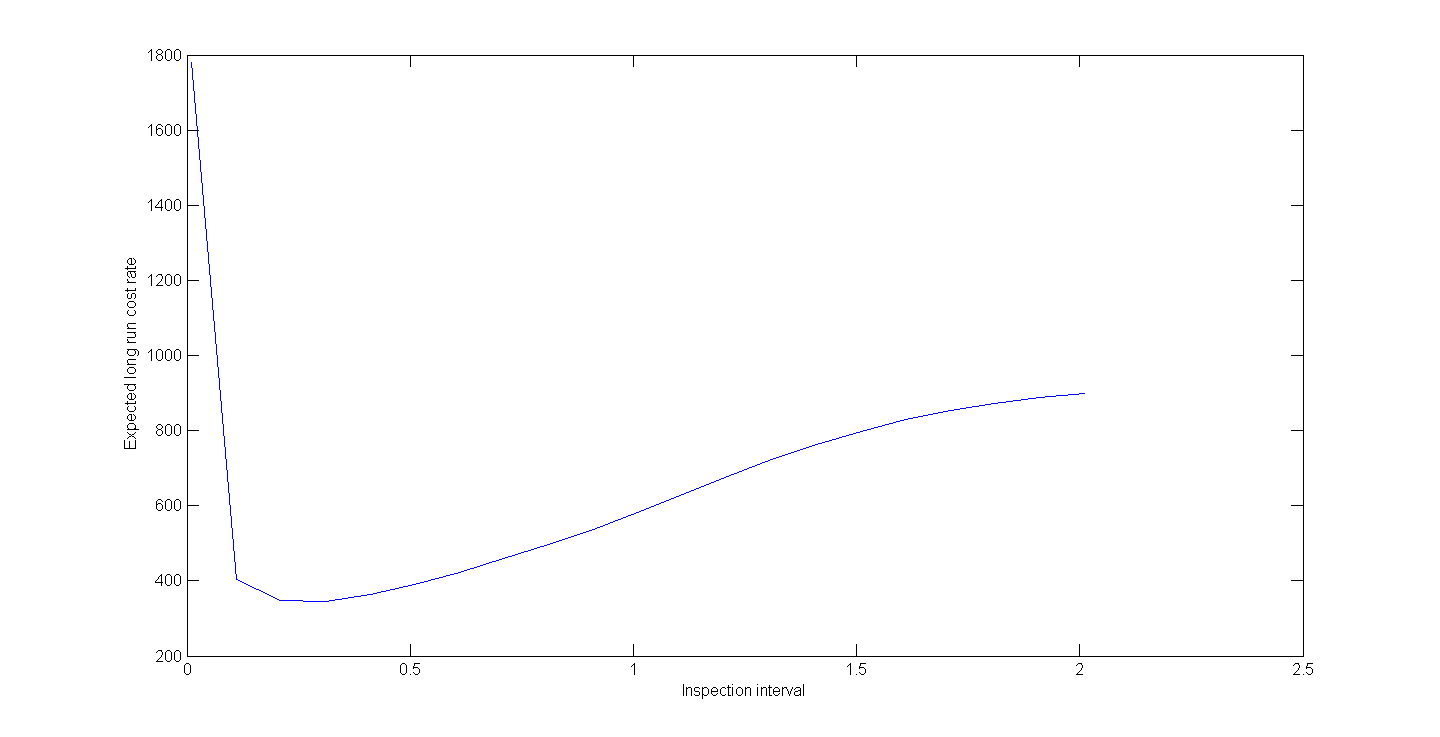
\includegraphics[width=6in]{example2.png}\\
  \footnotesize
  \caption{ \footnotesize{Expected cost per unit time v inspection interval} }\label{pic:example2}
\end{figure}

The optimal inspection interval is $0.3 \times 100=30$ days. 
\qed
\end{example}

\subsection{Conclusion}
In this section, we discussed two periodic inspection models for a single-component system based on the DTM \cite{Wang08}. Two examples are also proposed to demonstrate the numerical results of these two models.  

A master project that used the DTM in the analysis will be uploaded as a case study. Notice that the material of this case study is not required in the exam.
\subsection{Exercises}

\begin{exercise} \label{exercise:DTM1}
(level: standard)

The degradation of a machine can be described by a DTM. The engineers collect the time to defect data in the lab by doing reliability testings. The time to defect data statistically suggest that the time to defect follows an exponential distribution with $\lambda=1$. The time unit is one month. The engineers also collect the data about the duration from the defect time point till failure in the lab. The delay time seems to follow an uniform distribution according to the statistical fitting results. The cdf is given by
\begin{equation*}
F(t)=\dfrac{t}{10}, 0\leq t\leq 10.
\end{equation*} 
For this machine, we will apply a periodic inspection policy with a fixed inspection interval $\tau$. When we detect defects on the machine, we will replace the machine with a new one to prevent unexpected failures. Upon failures we will also replace the machine with a new one. The costs of a replacement are equal to EURO 3000. For a corrective maintenance
action additional costs equal to EURO 1000 are incurred because of the disturbance of the production process that depends on the availability of the machine. The inspection cost is 10 Euro.

Determine the average costs of the periodic inspection policy as a function of $\tau$ and determine the optimal policy and the corresponding average costs.
\end{exercise}

\begin{exercise} \label{exercise:DTM2}
(level: standard)

The degradation of a machine can be described by a DTM. The engineers collect the time to defect data in the lab by doing reliability testings. The time to defect data statistically suggest that the time to defect follows an uniform distribution. The cdf is given by
\begin{equation*}
F(t)=\dfrac{t}{10}, 0\leq t\leq 10.
\end{equation*} 
The time unit is one month. The engineers also collect the data about the duration from the defect time point till failure in the lab. The delay time seems to follow an exponential distribution with $\lambda=1$ according to the statistical fitting results.  
For this machine, we will apply a periodic inspection policy with a fixed inspection interval $\tau$. When we detect defects on the machine, we will replace the machine with a new one to prevent unexpected failures. Upon failures we will also replace the machine with a new one. The costs of a replacement are equal to EURO 3000. For a corrective maintenance
action additional costs equal to EURO 1000 are incurred because of the disturbance of the production process that depends on the availability of the machine. The inspection cost is 10 Euro.

Determine the average costs of the periodic inspection policy as a function of $\tau$ and determine the optimal policy and the corresponding average costs.
\end{exercise}

\begin{exercise}
(level: above standard)

Reconsider Exercise \ref{exercise:DTM1} and \ref{exercise:DTM2}. 
\begin{enumerate}
\item Is the periodic inspection policy with a fixed inspection interval suitable for the two cases in your opinion? Pls state the reasons.
\item Could you propose an inspection policy that is more appropriate than the current policy? Pls give the mathematical formulations of your own inspection policy. (hint: derive the $E[CL]$ and $E[CC]$)
\end{enumerate}

\end{exercise}


\section{Degradation Models}

If the degradation of the condition of a component or a system can be described as a stochastic process over time, we can propose maintenance models based on the probability models of the degradation processes. There are many degradation processes that can be used to describe the changes of the condition of a component or a system. To specify which degradation process is the most appropriate one, we first have to collect information of the failure or degradation mechanism of the component or the system. Hopefully we can get the basic characteristics of the degradation mechanism to screen out the not-appropriate degradation models. The degradation data can be obtained from the reliability testings in labs or from the operating fields. Statistical techniques should be used to estimate the parameters of the degradation models and do the fitting test. Then a suitable degradation model can be selected. For a literature review on the degradation models, see \cite{ZhuPengvanHoutum14}. 

In this section, we consider the cases for which the condition of a component can be represented by one variable. Then a stochastic process $\{X(t),t\geq 0\}$ can describe the degradation process of the condition of a component. If the degradation level $X(\cdot)$ passes a certain failure limit $H$, as shown in Figure \ref{pic:degradation1}, we assume that a failure will happen. This failure can be either a \textit{soft failure} or a \textit{hard failure}. We define a \textit{soft failure} as a failure that will not stop the operation of a system immediately, but will incur extra costs, such as quality loss cost or low performance cost. A \textit{hard failure} is a failure that will stop the operation of a system immediately. 

\begin{figure}[h!!!]  % ��ͼ���� i
  % Requires \usepackage{graphicx}
  \centering
  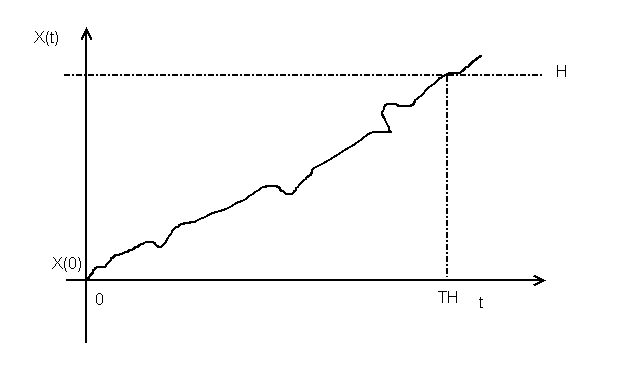
\includegraphics[width=6in]{Degradation1.png}\\
  \footnotesize
  \caption{ \footnotesize{Illustration of a degradation process} }\label{pic:degradation1}
\end{figure}

Here are several examples of degrading systems.

\begin{example}\label{ex:Degradation1} \renewcommand{\qedsymbol}{$\lozenge$} \mbox{}  

\begin{enumerate}
\item Consider a Micro-Electro-Mechanical System (MEMS) containing one microengine that is subject to wear, see Figure \ref{pic:degradation2}.  Furthermore, the failure of the microengine causes the failure of the system.  The failure of the microengine occurs when the wear volume of material reaches a critical threshold.  The wear volume of material can be estimated by measuring the volume of the wear debris or the missing volume in the worn device.  For example, a Focused Ion Beam system is effective to evaluate the amount of wear debris by producing cross sections of the precise area of interest in MEMS structures \cite{PengFengCoit09}.

\begin{figure}[h!!!]  % ��ͼ���� i
  % Requires \usepackage{graphicx}
  \centering
  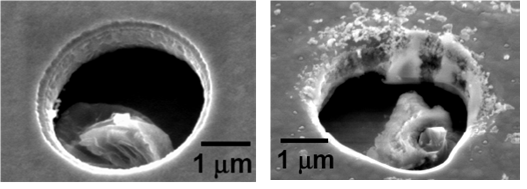
\includegraphics[width=6in]{Degradation2.png}\\
  \footnotesize
  \caption{ \footnotesize{Undamaged and severe damaged pin holes in a drive gear} }\label{pic:degradation2}
\end{figure}

\item For light display devices, such as plasma display panels (PDPs), vacuum fluorescent displays (VFDs) and fluorescent lamps (FLs), the critical performance characteristic is the luminosity that is related to brightness. Failure of such devices has been traditionally defined in terms of the degradation in luminosity over time. For example, the industry standard definition for PDP lifetime is the time at which the PDP luminosity falls below $50\%$ of its initial luminosity. Failure of FLs is defined as the time when a lamp’s luminosity falls below $60\%$ of its luminosity. \cite{FengPengCoit10}.

\end{enumerate}
\qed
\end{example}
  
\subsection{A control-limit policy for a single-component system}
We consider a CBM policy under which a condition measurement is recorded periodically, and once the measurement is higher than a control limit, repair or replacement of the component may be initiated. Our goal is to optimize the control limit and monitoring interval by minimizing the expected total cost rate.

The condition of the monitored item deteriorates over time. Such deterioration may be estimated based on the condition monitoring data that are collected at the monitoring intervals. There are two levels on the degradation process that influence the maintenance actions. The first level is the control limit, denoted by $C$. Once the deterioration is equal to or higher than this level, the item will be replaced by a new one. The second level is the failure limit $H$. If the deterioration of the item has reached the failure limit, it will incur a \textit{hard failure}. This failure limit is usually known and fixed in practice. Upon such failures, the item will also be replaced by a new one. Figure \ref{pic:degradation3} demonstrates the policy. The first passage time of the degradation process $\{X(t),t\geq 0\}$ over the control limit $C$ is denoted by $T_{C}$, which can be derived when the degradation process is specified to be a certain stochastic process. The first passage time of the degradation process over the failure limit $H$ is denoted by $T_{H}$, which can also be derived similarly.

\begin{figure}[h!!!]  % ��ͼ���� i
  % Requires \usepackage{graphicx}
  \centering
  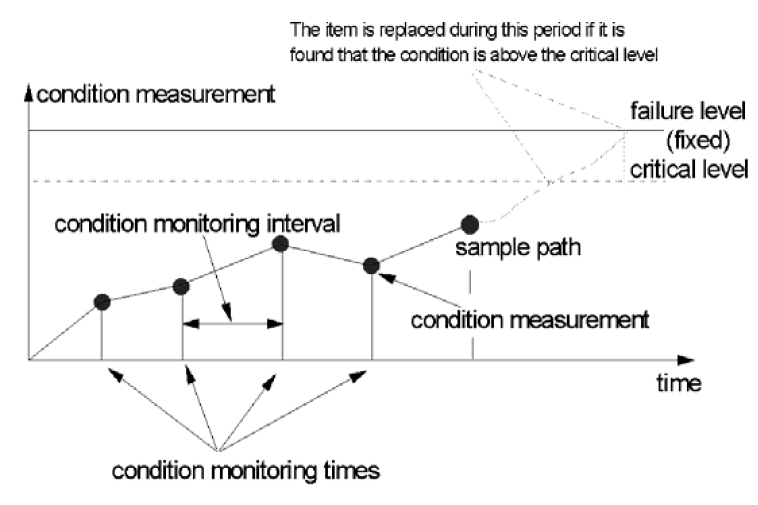
\includegraphics[width=6in]{Degradation3.png}\\
  \footnotesize
  \caption{ \footnotesize{Illustration of a CBM policy for a single-component system} }\label{pic:degradation3}
\end{figure} 

We assume the replacement time is negligible compared with the lifetime of the item. If the item gets replaced by a new one, the monitoring schedule restarts after the replacement. Then the replacement time points are renewal points in the analysis. 

A renewal cycle may span several monitoring intervals. Following the previous analysis procedure of renewal theory, we distinguish two renewal events, i.e., the failure renewal and the inspection renewal when the degradation level is above the control limit but below the failure limit. We are interested in the probabilities of the two renewal events. The probability that the failure renewal occurs in a certain monitoring interval $((i-1)\tau,i\tau)$ is the probability that the degradation level first passes the failure limit in the monitoring interval $((i-1)\tau,i\tau)$ and the degradation level first passes the control limit after the time point $(i-1)\tau$ (otherwise the component will be replaced according to our CBM policy), i.e.,
\begin{align*}
& Pr((i-1)\tau<T_{H}<i\tau \cap (i-1)\tau<T_{C}<i\tau ) \nonumber \\
& = \int_{(i-1)\tau}^{i\tau} f_{T_{C}}(u) F_{T_{H}|T_{C}=u}(i\tau)du. 
\end{align*} 
where $f_{T_{C}}(\cdot)$ is the probability density function of $T_{C}$ and $F_{T_{H}|T_{C}=u}(\cdot)$ is the cumulative distribution function of $T_{H}$ given that $T_{C}=u$. 
The probability that the inspection renewal with replacement occurs at time point $i\tau$ is the probability that the degradation level does not cross the failure limit till $i\tau$ and the degradation level crosses the control limit after the time point $(i-1)\tau$ (otherwise the component will be replaced at $(i-1)\tau$), i.e.,
\begin{align*}
& Pr(T_{H}\geq i\tau \cap (i-1)\tau<T_{C}<i\tau ) \nonumber \\
& = \int_{(i-1)\tau}^{i\tau} f_{T_{C}}(u) (1-F_{T_{H}|T_{C}=u}(i\tau))du. 
\end{align*} 

The failure renewals and the inspection renewals can happen at any monitoring interval. Notice that the summation of the probability of the failure renewal and the probability of the inspection renewal over all the possible inspection intervals is equal to one,
\begin{align*}
& \sum_{i=1}^{\infty} \Bigg\{Pr((i-1)\tau<T_{H}<i\tau \cap (i-1)\tau<T_{C}<i\tau )+Pr(T_{H}\geq i\tau \cap (i-1)\tau<T_{C}<i\tau ) \Bigg\} \nonumber \\
& = \sum_{i=1}^{\infty} \Bigg\{ \int_{(i-1)\tau}^{i\tau} f_{T_{C}}(u) F_{T_{H}|T_{C}=u}(i\tau)du+\int_{(i-1)\tau}^{i\tau} f_{T_{C}}(u) (1-F_{T_{H}|T_{C}=u}(i\tau))du \Bigg\} \nonumber \\
& = 1. 
\end{align*}
Then based on the analysis of these two renewal events, the renewal cycle length is
\begin{align} \label{eq:model3cyclelength}
E[CL]= \sum_{i=1}^{\infty} \Bigg\{ \int_{(i-1)\tau}^{i\tau} t \int_{(i-1)\tau}^{i\tau} f_{T_{C}}(u) f_{T_{H}|T_{C}=u}(t)du dt + i\tau \int_{(i-1)\tau}^{i\tau} f_{T_{C}}(u) (1-F_{T_{H}|T_{C}=u}(i\tau)) du \Bigg\}.  
\end{align}
where $f_{T_{H}|T_{C}=u}(\cdot)$ is the probability density funciton of $T_{H}$ given that $T_{C}=u$.
For the renewal cycle cost, when the failure renewal happens in an inspection interval $((i-1)\tau,i\tau)$, the renewal cycle cost equals the sum of the inspection cost $(i-1)C_{i}$ and the corrective maintenance cost $C_{cm}$. Then the expected cycle cost due to failure renewals is
\begin{align} \label{eq:model3cyclecost1}
& \sum_{i=1}^{\infty} \Bigg\{((i-1)C_{i}+C_{cm})Pr((i-1)\tau<T_{H}<i\tau \cap (i-1)\tau<T_{C}<i\tau ) \Bigg\} \nonumber \\
& = \sum_{i=1}^{\infty} \Bigg\{ ((i-1)C_{i}+C_{cm})\int_{(i-1)\tau}^{i\tau} f_{T_{C}}(u) F_{T_{H}|T_{C}=u}(i\tau)du \Bigg\}  
\end{align} 
When the inspection renewal happens at time point $i\tau$, the renewal cycle cost equals the sum of the inspection cost $iC_{i}$ and the preventive maintenance cost $C_{pm}$. Then the expected cycle cost due to inspection renewals is
\begin{align} \label{eq:model3cyclecost2}
& \sum_{i=1}^{\infty} \Bigg\{(iC_{i}+C_{pm})Pr(T_{H}\geq i\tau \cap (i-1)\tau<T_{C}<i\tau ) \Bigg\} \nonumber \\
& = \sum_{i=1}^{\infty} \Bigg\{ (iC_{i}+C_{pm})\int_{(i-1)\tau}^{i\tau} f_{T_{C}}(u) (1-F_{T_{H}|T_{C}=u}(i\tau))du \Bigg\}  
\end{align}
Therefore, the expected renewal cycle cost can be obtained by summing Equation \ref{eq:model3cyclecost1} and \ref{eq:model3cyclecost2},
\begin{align} \label{eq:model3cyclecost}
 E[CC] \nonumber \\
 =\sum_{i=1}^{\infty} \Bigg\{ & ((i-1)C_{i}+C_{cm})Pr((i-1)\tau<T_{H}<i\tau \cap (i-1)\tau<T_{C}<i\tau ) \nonumber \\
 & + (iC_{i}+C_{pm})Pr(T_{H}\geq i\tau \cap (i-1)\tau<T_{C}<i\tau ) \Bigg\} \nonumber \\
 = \sum_{i=1}^{\infty} \Bigg\{ & ((i-1)C_{i}+C_{cm})\int_{(i-1)\tau}^{i\tau} f_{T_{C}}(u) F_{T_{H}|T_{C}=u}(i\tau)du \nonumber \\
 & +(iC_{i}+C_{pm})\int_{(i-1)\tau}^{i\tau} f_{T_{C}}(u) (1-F_{T_{H}|T_{C}=u}(i\tau))du \Bigg\}  
\end{align}
According to the renewal theory, the expected long run cost rate can be obtained by Equation \ref{eq:renew},\ref{eq:model3cyclelength} and \ref{eq:model3cyclecost}.

\subsection{First passage time: random coefficient model}
The above CBM policy requires the derivation of the distributions of first passage time and the condition first passage time. Random coefficient model is one type of probability models to describe the degradation process of a component \cite{ZhuPengvanHoutum14}. In this subsection we will derive the first passage time and the condition first passage time based on a given random coefficient model. For a random coefficient model, the degradation path can be described by a function over time that has fixed coefficients and random coefficients, $X(t;\Phi,\Theta)$, given a set of constant parameters $\Phi=\{\phi_{1}, \cdots, \phi_{Q}\}, Q \in \mathbb Z_{> 0} $ and a set of random parameters, $\Theta=\{\theta_{1}, \cdots, \theta_{V}\}, V \in \mathbb Z_{> 0} $, following certain probability distributions. The random parameters describe the unit-to-unit variations (instead of the temporal variations). Then clearly, the probability that the first passage time $T_{\chi}$ over a threshold $\chi$  is less than time $t$ is equal to the probability that the maximum degradation level in time interval $[0,t]$ is larger than the threshold $\chi$ 
\begin{equation} \label{eq:degradation2.1}
Pr\{T_{\chi}< t\}=Pr\{\max_{0\leq u\leq t} X(u)> \chi \}.
\end{equation}
The conditional distribution of first passage time $T_{\chi_{2}}$ given that the first passage time of $\chi_{1} (< \chi_{2})$ is at time point $s$ is equal to
\begin{equation} \label{eq:degradation2.2}
Pr\{T_{\chi_{2}}< t | T_{\chi_{1}}=s \}=Pr\{\max_{0\leq u\leq t} X(u)> \chi_{2} | X(s)=\chi_{1} \cap \arg \max_{0\leq u\leq s} X(u) =s\}. 
\end{equation}

\begin{example} \label{ex:degradation1} \renewcommand{\qedsymbol}{$\lozenge$} \mbox{} 
Consider a component in a system with a degradation path $X(t;\Phi,\Theta)=\phi_{1}+\theta_{1}t$ where $\Phi=\{\phi_{1}\}$ and $\Theta=\{\theta_{1}\}$. Equation \ref{eq:degradation2.1} can be written in terms of $F_{\theta_{1}}$ (the cumulative density function of random variable $\theta_{1}$, $\theta_{1} > 0$),
\begin{eqnarray} 
Pr\{T_{\chi} <t\}  & = & Pr\{\phi_{1}+\theta_{1}t > \chi \} \notag\\
 & = &  Pr\{\theta_{1} > \frac{\chi-\phi_{1}}{t} \} \notag\\
& = & 1- F_{\theta_{1}}\Big( \frac{\chi-\phi_{1}}{t}\Big). \notag\\
\end{eqnarray}

Since the randomness is from the unit-to-unit variation, when we know that $T_{\chi_{1}}$ is $s$, it is equivalent to say that this component has a degradation rate $\theta_{1}=\dfrac{\chi_{1}-\phi_{1}}{s}$. Therefore, given that $T_{\chi_{1}}$ is $s$, the conditional probability mass function of $T_{\chi_{2}}$ is

\begin{equation*}
Pr\{T_{\chi_{2}}=\dfrac{(\chi_2-\phi_1)s}{\chi_1-\phi_1} | T_{\chi_{1}}=s \} =1.
\end{equation*} 
In other words, $T_{\chi_2}$ is a constant number $\dfrac{(\chi_2-\phi_1)s}{\chi_1-\phi_1}$ given that $T_{\chi_1}$ is $s$.

An illustration of this linear random coefficient model is given in Figure \ref{pic:example3}.
\begin{figure}[h!!!]  % ��ͼ���� i
  % Requires \usepackage{graphicx}
  \centering
  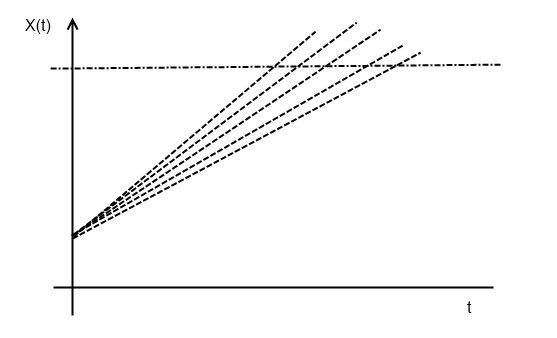
\includegraphics[width=6in]{example3.png}\\
  \footnotesize
  \caption{ \footnotesize{The linear random coefficient model} }\label{pic:example3}
\end{figure}

If $\phi_1=1$ and $\theta_1\sim Exponential (\lambda=1)$, then, when $\chi_1=2$, the first passage time over $\chi_1$ is
\begin{eqnarray} 
Pr\{T_{\chi_1} <t\}  & = & Pr\{1+\theta_{1}t > 2 \} \notag\\
 & = &  Pr\{\theta_{1} > \frac{2-1}{t} \} \notag\\
& = & 1- F_{\theta_{1}}\Big( \frac{2-1}{t}\Big) \notag\\
& = & 1- (1-exp(-\dfrac{1}{t})) \notag\\
& = & exp(-\dfrac{1}{t})
\end{eqnarray}
as shown in Figure \ref{pic:example3.2}.
\begin{figure}[h!!!]  % ��ͼ���� i
  % Requires \usepackage{graphicx}
  \centering
  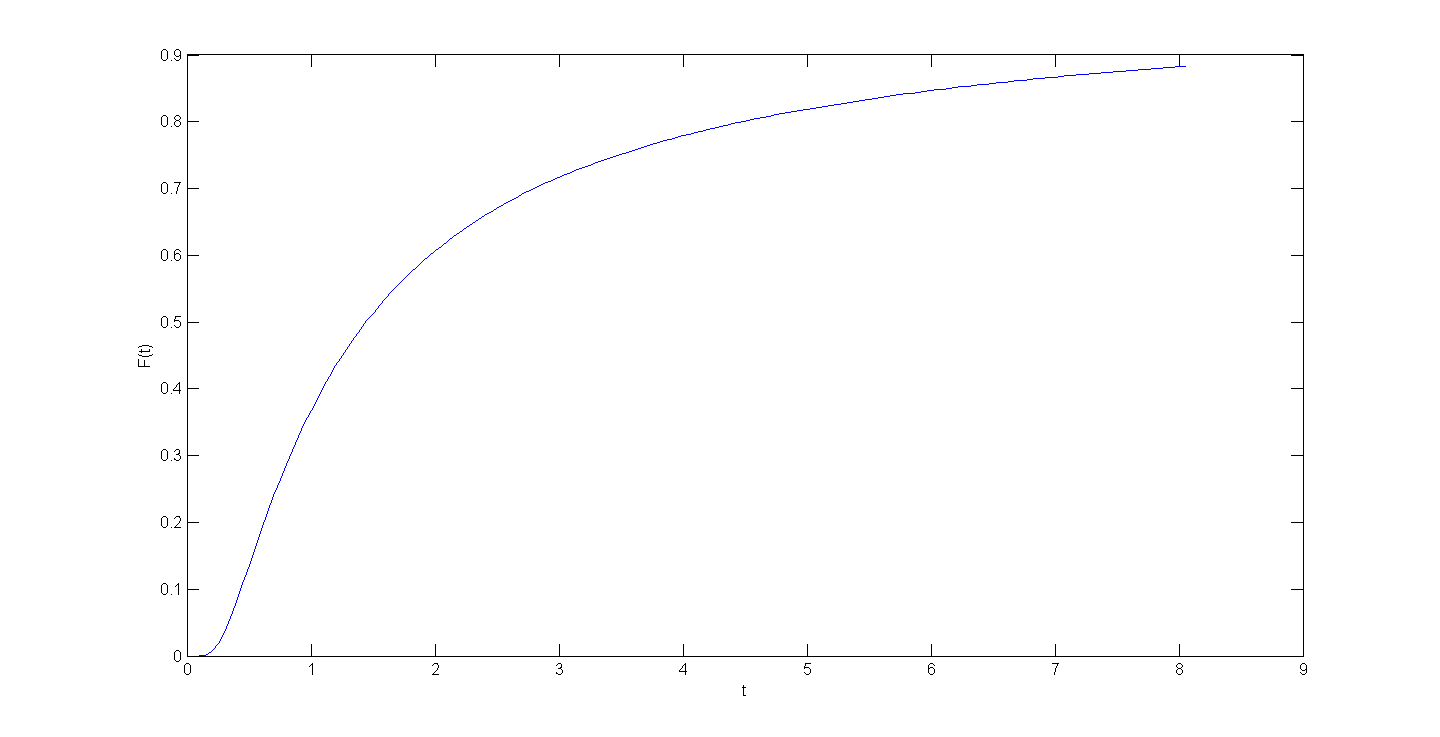
\includegraphics[width=6in]{example32.png}\\
  \footnotesize
  \caption{ \footnotesize{The cdf of the first passage time for a linear random coefficient model} }\label{pic:example3.2}
\end{figure}
If we know the first passage time $T_{\chi_1}=1$ and $\chi_2=3$, the conditional probability mass function of $T_{\chi_{2}}$ given that $T_{\chi_1}=1$ is

\begin{equation*}
Pr\{T_{\chi_{2}}=\dfrac{(3-1)1}{2-1} | T_{\chi_{1}}=1 \} =1.
\end{equation*} 

In other words, $T_{\chi_2}$ is a constant number $\dfrac{(3-1)1}{2-1}$ given that $T_{\chi_1}$ is 1.
 
\qed
\end{example}
\begin{example} \label{ex:degradation2} \renewcommand{\qedsymbol}{$\lozenge$} \mbox{}
Suppose the degradation path of a component can be described by a linear random coefficient model. This means $X(t)=1+\theta_1t$, $\theta_1 \sim Normal(\mu=1,\sigma=0.1)$. Suppose the failure limit of this degradation process $H$ is 5.

We consider a CBM policy under which a condition measurement is recorded periodically, and once the measurement is higher than a control limit, the component will be replaced by a new one.

The inspection cost is $C_i=15$. The corrective maintenance cost is $C_{cm}=1000$. The preventive maintenance cost is $C_{pm}=150$.

\begin{figure}  
  % Requires \usepackage{graphicx}
  \centering
  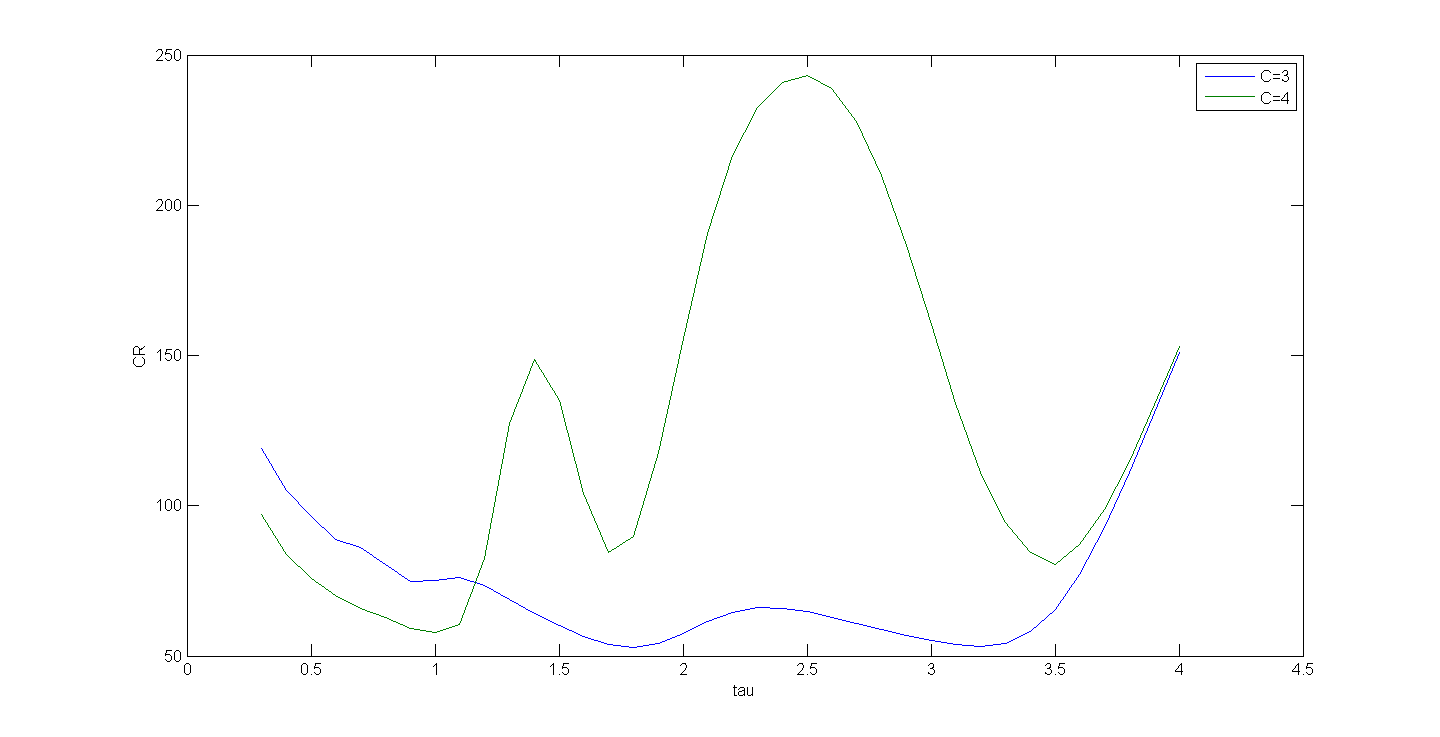
\includegraphics[width=6in]{example41.png}\\
  \footnotesize
  \caption{ \footnotesize{The average cost rate via tau when C=3 or 4} }\label{pic:example4.1}
\end{figure}
%
%


According to Equation \ref{eq:model3cyclelength}, the expected cycle length based on this linear random coefficient model is
\begin{align} \label{example:model3cyclelength}
E[CL]= \sum_{i=1}^{\infty} \Bigg\{  \int_{(i-1)\tau}^{i\tau} f_{T_{C}}(u) \dfrac{(H-\phi_1)u}{C-\phi_1}Pr(T_{H}<i\tau|T_{C}=u) du  + i\tau \int_{(i-1)\tau}^{i\tau} f_{T_{C}}(u) Pr(T_{H}\geq i\tau|T_{C}=u) du \Bigg\}.  
\end{align}
where if $\dfrac{(H-\phi_1)u}{C-\phi_1}<i\tau$,$Pr(T_{H}<i\tau|T_{C}=u) =1$, since the conditional $T_H$ is a constant number $\dfrac{(H-\phi_1)u}{C-\phi_1}$.
Using Equation \ref{eq:renew}, \ref{example:model3cyclelength} and \ref{eq:model3cyclecost}, the expected long run cost rate as a function of $\tau$ and $C$ is shown in Figure \ref{pic:example4.1} and \ref{pic:example4.2} (notice that it should be a 3D figure since there are two decision variables but in order to get some insights we choose the 2D figures).
\begin{figure}
  % Requires \usepackage{graphicx}
  \centering
  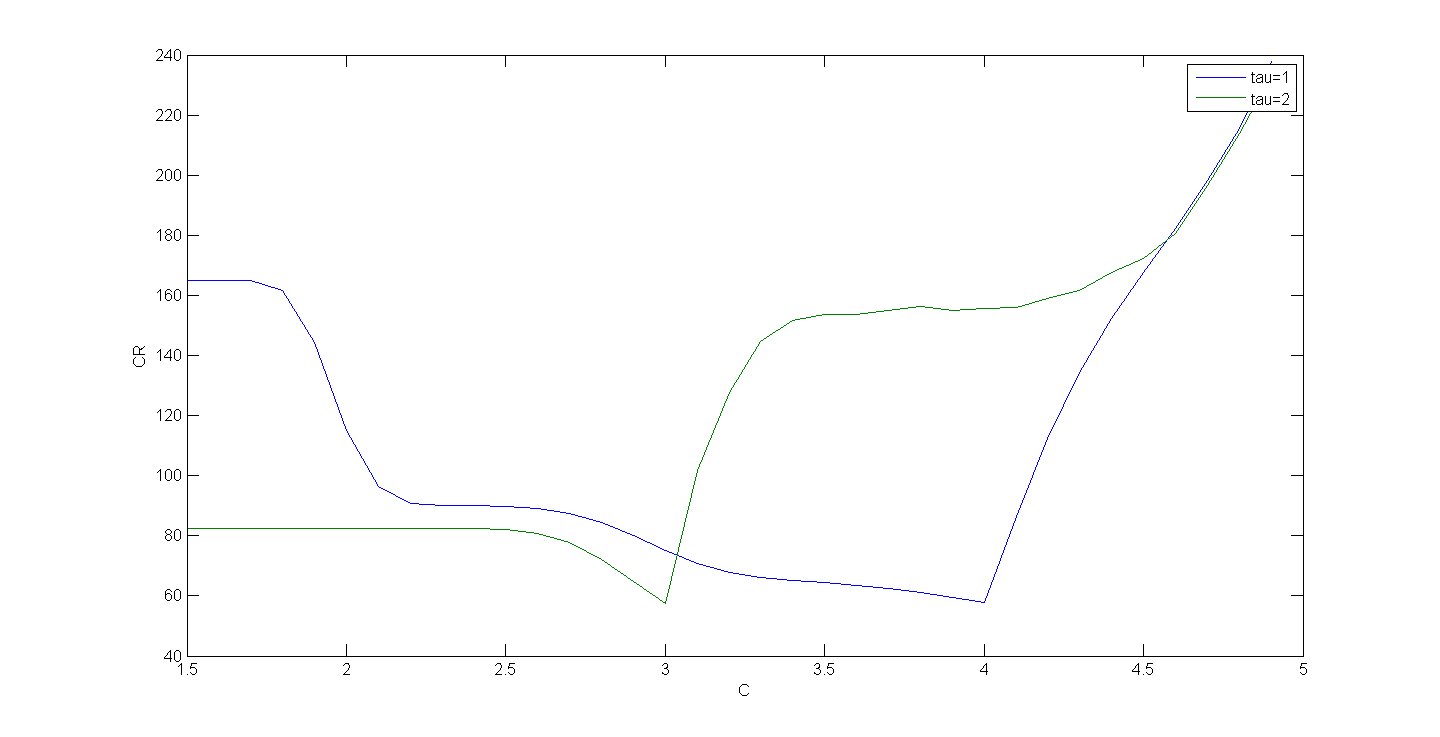
\includegraphics[width=6in]{example42.png}\\
  \footnotesize
  \caption{ \footnotesize{The average cost rate via C when tau=1 or 2} }\label{pic:example4.2}
\end{figure}

%\begin{figure}  
%  % Requires \usepackage{graphicx}
%  \centering
%  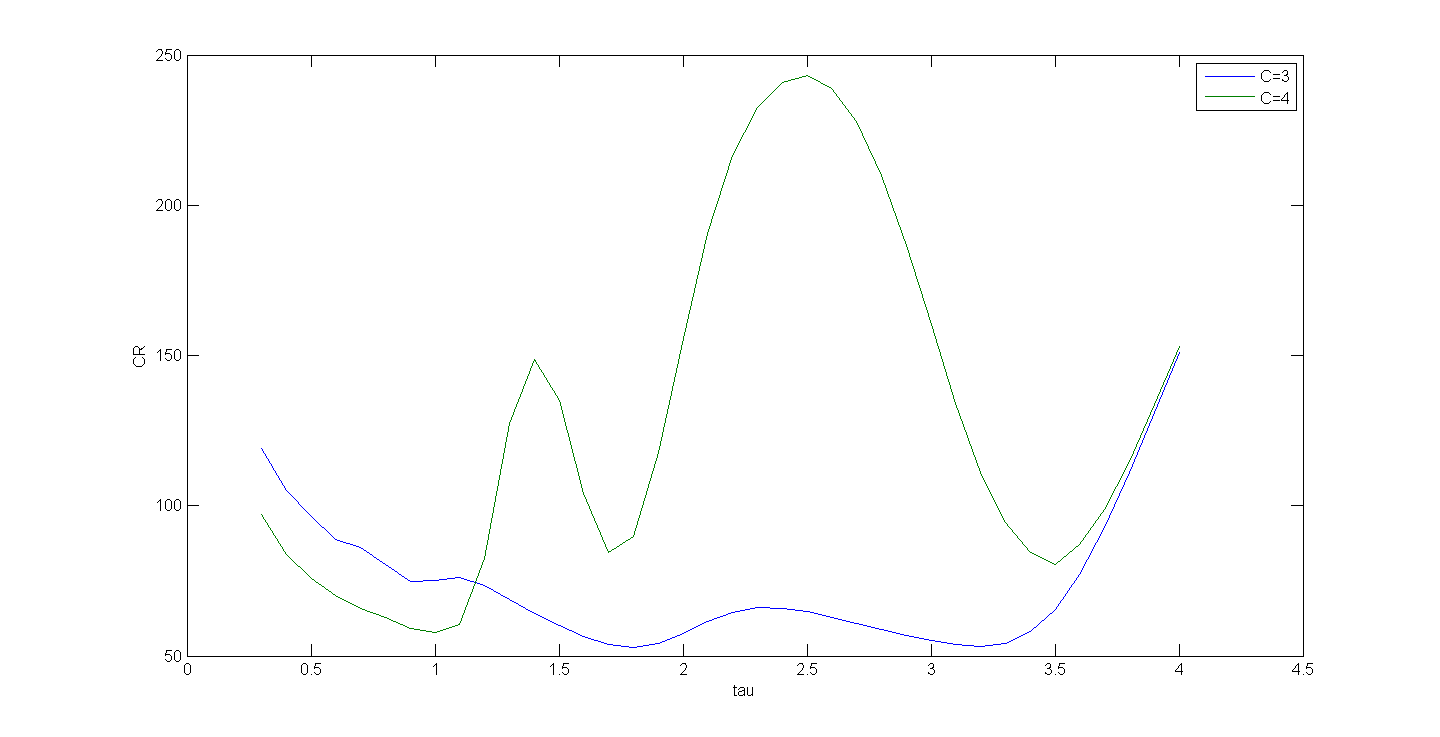
\includegraphics[width=6in]{example41.png}\\
%  \footnotesize
%  \caption{ \footnotesize{The average cost rate via tau when C=3 or 4} }\label{pic:example4.1}
%\end{figure}
%
%
%\begin{figure}
%  % Requires \usepackage{graphicx}
%  \centering
%  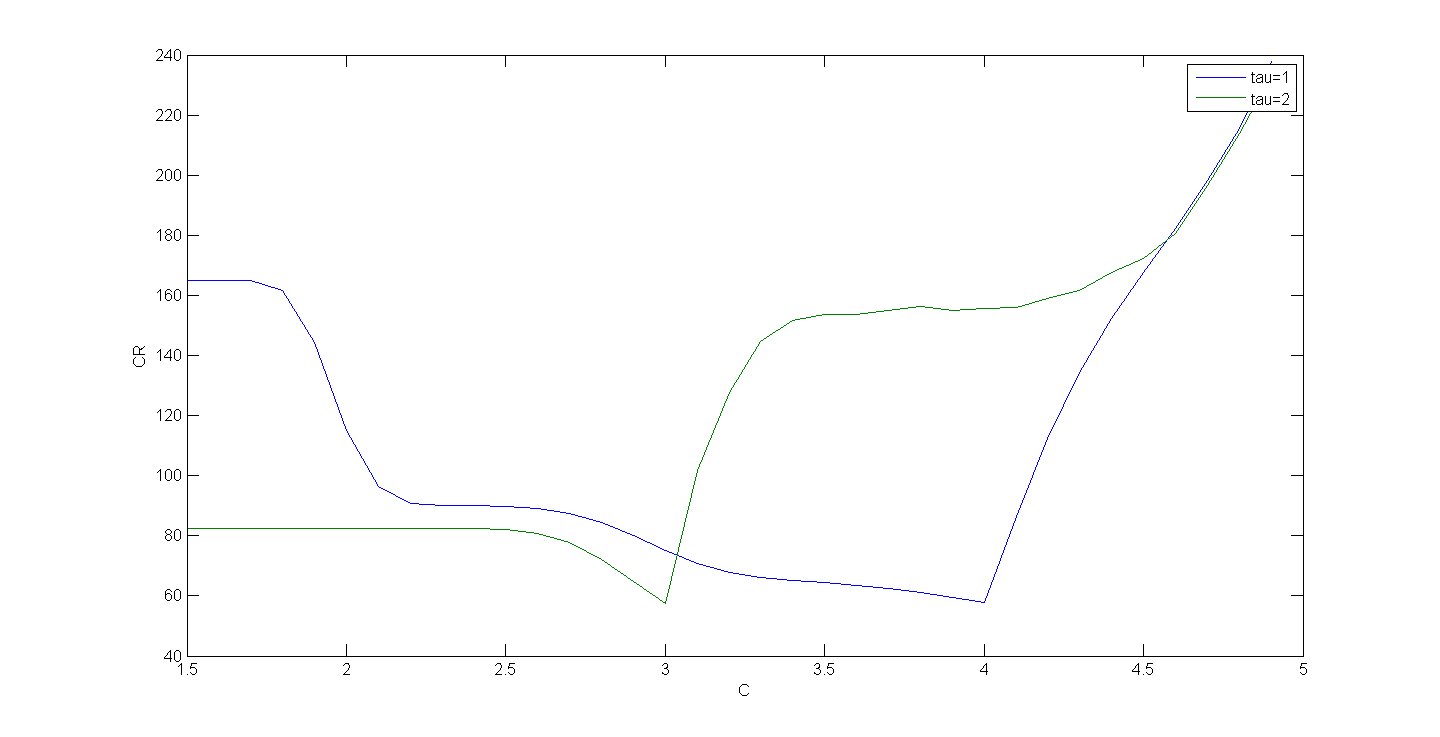
\includegraphics[width=6in]{example42.png}\\
%  \footnotesize
%  \caption{ \footnotesize{The average cost rate via C when tau=1 or 2} }\label{pic:example4.2}
%\end{figure}

\end{example}

\subsection{Conclusion}
In this section, we discussed one periodic inspection model for a single-component system subject to deterioration. We introduced one degradation model: random coefficient model and developed its first passage time. Two numerical examples are provided to show the random coefficient model and how to use it in the periodic inspection model.

A master project that used part of the material in this section will be uploaded as a case study. Notice that the material of this case study is not required in the exam.
\subsection{Exercises}

\begin{exercise} \label{exercise:Degradation1}
(level: standard)

The wear-out of a rotating part can be described by a a linear function, $X(t)=\theta t$. The time unit is one revolution. The wear-out can be determined by inspections on wear debris. Based on the wear-out mechanism, $\theta$ is dependent on the hardness of the material, the radius of the rotating part, and the force between rubbing surfaces. It is a random parameter among units. The engineers collect the degradation data of 80 units. For each unit, there's an estimated linear function through regression, which has an estimated $\hat{\theta}$. Then there are 80 $\hat{\theta}$ s. The engineers find out the distribution of $\theta$ is a normal distribution with mean $\hat{\mu_{\theta}}= 1$ and standard deviation $\hat{\sigma_{\theta}}= 0.1$, based on the 80 $\hat{\theta}$ s. The failure limit of the wear-out is given as $H=5000$. (the negative proportion of the normal distribution for $\theta$ can be ignored in the computation.)  

\begin{itemize}
 \item Suppose the engineers set a warning limit of $C=4000$. What is the cdf of the first passage time over $C$ for this degrading component?
 \item Conditioned on the fact that the wear-out of the rotating component at 3500 revolutions is 4000, what is the conditional first passage time over $H$?   
 \end{itemize} 
For this component, we will apply a periodic inspection policy with a fixed inspection interval $\tau$ and a control limit $C$. When the degradation level is above $C$ the component will get replaced. The degradation level can only be observed through inspections. Upon failures we will also replace the machine with a new one. The costs of a replacement are equal to EURO 3000. For a corrective maintenance action additional costs equal to EURO 1000 are incurred because of the disturbance of the production process that depends on the availability of the machine. The inspection cost is 10 Euro.

Determine the average long run cost rate of the periodic inspection policy as a function of $\tau$ and $C$. Determine the optimal policy and the corresponding average cost rate.
\end{exercise}

\begin{exercise} 
(level: standard)
It is known that the luminosity for several types of light displays decreases exponentially over the majority of the device life cycle (the time unit is one day), and the logarithm of the luminosity at time $t$, $X(t)$, can be expressed as 
\begin{equation*}
X(t)=ln \ \Lambda(t)=\phi-\theta t,
\end{equation*}
where $\Lambda(t)$ denotes the luminosity at time $t$, $\phi$ is the log-transformed initial luminosity, and $\theta$ is the rate of degradation. The log-transformed initial luminosity, $\phi$ is assumed to be a constant and the degradation rate   varies from unit-to-unit, which reasonably fits the lognormal distribution.

The engineers collect the degradation data of 80 units. The log-transformed initial luminosity is 5000 for all units or the whole population. For each unit, there's an estimated linear function through regression, which has an estimated $\hat{\theta}$. Then there are 80 $\hat{\theta}$ s. The engineers find out the lognormal distribution of $\theta$ has parameter $\hat{\mu}= 1$ and standard deviation $\hat{\sigma}= 0.2$, based on the 80 $\hat{\theta}$ s. Notice that the pdf of a lognormal distribution is
\begin{equation*}
f(x)=\dfrac{1}{x\sigma\sqrt{2\pi}}exp(\dfrac{-(ln \ x -\mu)^{2}}{2\sigma^{2}})
\end{equation*}
The cdf of a lognormal distribution is
\begin{equation*}
F(x)=\Phi(\dfrac{ln \ x -\mu}{\sigma}).
\end{equation*}

The failure limit of the illumination degradation is given as $H=1000$. 
\begin{itemize}
 \item Suppose the engineers set a warning limit of $C=2000$. What is the cdf of the first passage time over $C$ for this degrading component?
 \item Conditioned on the fact that the logarithm of the illumination of this component at time point 3500 is 2000, what is the first passage time over $H$?   
 \end{itemize} 

\end{exercise}

\begin{exercise}\label{exercise:degradation2}
(level: above standard)

Reconsider Exercise \ref{exercise:degradation2}. 
For this component, we will apply a periodic inspection policy with a fixed inspection interval $\tau$ and a control limit $C$. When the degradation level is under $C$ the component will get replaced. The degradation level can be measured through inspections. \emph{The failures are not self-announcing}, which will also be detected by inspections when the degradation level is below the failure limit $H$. Upon failures we will also replace the machine with a new one. The costs of a replacement are equal to EURO 3000. For a corrective maintenance action additional costs equal to EURO 1000 are incurred because of the disturbance of the production process that depends on the availability of the machine. The inspection cost is 10 Euro.

Determine the average long run cost rate of the periodic inspection policy as a function of $\tau$ and $C$. Determine the optimal policy and the corresponding average cost rate. (hint: derive $E[CC]$ and $E[CL]$)

\end{exercise}

\section{Appendices}

\begin{appendices}
\section{Numerical calculation for Example \ref{ex:DTM1}}
Matlab code for function $CR(\tau)$.
\begin{verbatim}
function CR=CR(tau)
lambda_X=0.6;
lambda_H=0.75;
Ccm=1000;
Cpm=150;
Ci=15;

    
% fXH=lambda_X*lambda_H/(lambda_H-lambda_X)*(exp(-lambda_X*t)-exp(-lambda_H*t));
% FXH=1+(-lambda_H*exp(-lambda_X*t)+lambda_X*exp(-lambda_H*t))/(-lambda_X+lambda_H);

    function int_term1_ECL=int_term1_ECL(t)
        int_term1_ECL=t.*(lambda_X.*lambda_H./(lambda_H-lambda_X).*(exp(-lambda_X.*t)-exp(-lambda_H.*t)));
    end

    


ECL=quad(@int_term1_ECL,0,tau)+tau*(1-(1+(-lambda_H*exp(-lambda_X*tau)+lambda_X*exp(-lambda_H*tau))/(-lambda_X+lambda_H)));

Prfailure=1+(-lambda_H*exp(-lambda_X*tau)+lambda_X*exp(-lambda_H*tau))/(-lambda_X+lambda_H);
Prinspectionwithoutreplacement=1-(1-exp(-lambda_X*tau));
Prinpsectionwithreplacement=lambda_X/(-lambda_X+lambda_H)*(exp(-lambda_X*tau)-exp(-lambda_H*tau));

ECC=Ccm*Prfailure+Ci*Prinspectionwithoutreplacement+(Cpm+Ci)*Prinpsectionwithreplacement;

CR=ECC/ECL;
end
\end{verbatim}
Matlab code for plotting function $CR(\tau)$.
\begin{verbatim}
i=1;
t(i)=0.1;
Re2(i)=CR(t(i));
while (t(i)<2.3)
    t(i+1)=t(i)+0.05;
    i=i+1;
    Re2(i)=CR(t(i));
end

plot(t,Re2)
\end{verbatim}
\section{Numerical calculation for Example \ref{ex:DTM2}}
Matlab code for evaluating $E[CL],E[CC]$ and $CR(\tau)$.
\begin{verbatim}
classdef m2gp2
    % Class for evaluation of Model 2
 
    properties
        % Default parameters
        
       beta_X=2;
eta_X=0.6;
beta_H=2;
eta_H=0.75;
Ccm=1000;
Cpm=150;
Ci=15;
    end  
    methods
        function obj = m2gp2(beta_X,eta_X,beta_H,eta_H,Ccm,Cpm,Ci)
            if nargin > 0
         
                obj.beta_X   = beta_X;
                obj.eta_X    = eta_X;
     obj.beta_H=beta_H;
     obj.eta_H=eta_H;
     obj.Ccm=Ccm;
     obj.Cpm=Cpm;
                obj.Ci=Ci;
            
            end
        end
        function y = pdfweibull_X(m2,x)
            if (x>=0)
     y=m2.beta_X.*(x.^(m2.beta_X-1))./(m2.eta_X.^m2.beta_X).*exp(-(x./m2.eta_X).^m2.beta_X);
            else y=0;
            end
        end
         function y = cdfweibull_X(m2,t)
            
            int = @(x) (m2.pdfweibull_X(x));
            y = quadgk(int,0,t,'MaxIntervalCount',100,'AbsTol',1.e-2);
         end
        function y = pdfweibull_H(m2,x)
            if (x>=0)
     y=m2.beta_H.*(x.^(m2.beta_H-1))./(m2.eta_H.^m2.beta_H).*exp(-(x./m2.eta_H).^m2.beta_H);
            else y=0;
            end
        end
         function y = cdfweibull_H(m2,t)
            
            int = @(x) (m2.pdfweibull_H(x));
            y = quadgk(int,0,t,'MaxIntervalCount',100,'AbsTol',1.e-2);
         end
         function y=ECL_i_1(m2,i,tau)
              function z=f_outer(t)
                z=zeros(size(t));
                for j=1:length(t)
                    a=(i-1).*tau;
                    b=i.*tau;
            f_inner=@(u)(m2.pdfweibull_X(u).*m2.pdfweibull_H(t(j)-u));
            z(j)=quadgk(f_inner,a,b,'MaxIntervalCount',100,'AbsTol',1.e-2).*...
                t(j);
                end
            end
            y=quadgk(@f_outer,(i-1).*tau,i.*tau,...
                'MaxIntervalCount',100,'AbsTol',1.e-2);
         end
         function y=ECL_i_2(m2,i,tau)
   
           function z=f_outer(t)
                z=zeros(size(t));
                for j=1:length(t)
                    
            z(j)=m2.pdfweibull_X(t(j)).*(1-m2.cdfweibull_H(i.*tau-t(j)));
                end
            end
            y=i.*tau.*quadgk(@f_outer,(i-1).*tau,i.*tau,...
                'MaxIntervalCount',100,'AbsTol',1.e-2);
         end
          function y=ECL(m2,tau)
            delta=1e-10;
            i=1;
            sum_1=0;
            sum_2=m2.ECL_i_1(i,tau)+m2.ECL_i_2(i,tau);
            while (sum_2-sum_1)>delta
                i=i+1;
                sum_1=sum_2;
                sum_2=sum_1+m2.ECL_i_1(i,tau)+m2.ECL_i_2(i,tau);
            end
            y=sum_2;
          end
        
         function y=ECC_i_1(m2,i,tau)
          
           function z=f_outer(t)
                z=zeros(size(t));
                for j=1:length(t)
                    
            z(j)=m2.pdfweibull_X(t(j)).*m2.cdfweibull_H(i.*tau-t(j));
                end
            end
            y=((i-1).*m2.Ci+m2.Ccm).*quadgk(@f_outer,(i-1).*tau,i.*tau,...
                'MaxIntervalCount',100,'AbsTol',1.e-2);
         end
         
         function y=ECC_i_2(m2,i,tau)
          
          function z=f_outer(t)
                z=zeros(size(t));
                for j=1:length(t)
                    
            z(j)=m2.pdfweibull_X(t(j)).*(1-m2.cdfweibull_H(i.*tau-t(j)));
                end
            end
            y=(i.*m2.Ci+m2.Cpm).*quadgk(@f_outer,(i-1).*tau,i.*tau,...
                'MaxIntervalCount',100,'AbsTol',1.e-2);
         end
              function y=ECC(m2,tau)
            delta=1e-10;
            i=1;
            sum_1=0;
            sum_2=m2.ECC_i_1(i,tau)+m2.ECC_i_2(i,tau);
            while (sum_2-sum_1)>delta
                i=i+1;
                sum_1=sum_2;
                sum_2=sum_1+m2.ECC_i_1(i,tau)+m2.ECC_i_2(i,tau);
            end
            y=sum_2;
              end
              function y=CR(m2,tau)
                  y=m2.ECC(tau)./m2.ECL(tau);
              end
        
    end
end


\end{verbatim}
Matlab code for plotting $CR(\tau)$.
\begin{verbatim}
% Clear
clear

% Parameters    
beta_X=2;
eta_X=0.6;
beta_H=2;
eta_H=0.75;
Ccm=1000;
Cpm=150;
Ci=15;

Be=m2gp2(beta_X,eta_X,beta_H,eta_H,Ccm,Cpm,Ci);
i=1;
t(i)=0.01;
Re2(i)=Be.CR(t(i));
while (t(i)<(2))
    t(i+1)=t(i)+0.1;
    i=i+1;
    Re2(i)=Be.CR(t(i));

end
 
plot(t,Re2)
\end{verbatim}
\section{Numerical calculation for Exercise \ref{exercise:DTM2}}
Matlab code for evaluating $E[CL],E[CC]$ and $CR(\tau)$.
\begin{verbatim}
classdef m2gp2Exercise2
   
    properties
        % Default parameters
        
       U_X=10;
lambda_H=1;
Ccm=4000;
Cpm=3000;
Ci=10;
    end  
    methods
        function obj = m2gp2Exercise2(U_X,lambda_H,Ccm,Cpm,Ci)
            if nargin > 0
         
                obj.U_X   = U_X;
                obj.lambda_H    = lambda_H;
     
     obj.Ccm=Ccm;
     obj.Cpm=Cpm;
                obj.Ci=Ci;
            
            end
        end
        function y = pdfuniform_X(m2,x)
     if (x<=m2.U_X)
         y=1./m2.U_X;
     else
         y=0;
     end
        end

        function y = pdfexponential_H(m2,x)
            if (x>=0)
     y=m2.lambda_H.*exp(-m2.lambda_H.*(x));
            else y=0;
            end
        end
         function y = cdfexponential_H(m2,t)
       
            
            
            int = @(x) (m2.pdfexponential_H(x));
            y = quadgk(int,0,t,'MaxIntervalCount',100,'AbsTol',1.e-2);
         end
         

         
         function y=ECL_i_1(m2,i,tau)
              function z=f_outer(u)
                z=zeros(size(u));
                for j=1:length(u)
                    
                    b=i.*tau;
            f_inner=@(t)(t.*m2.pdfexponential_H(t-u(j)));

            z(j)=m2.pdfuniform_X(u(j)).*quadgk(f_inner,u(j),b,'MaxIntervalCount',100,'AbsTol',1.e-2);

                end
            end
            y=quadgk(@f_outer,(i-1).*tau,i.*tau,...
                'MaxIntervalCount',100,'AbsTol',1.e-2);
         end
         
         
         
         function y=ECL_i_2(m2,i,tau)
   
           function z=f_outer(t)
                z=zeros(size(t));
                for j=1:length(t)
                    
            z(j)=m2.pdfuniform_X(t(j)).*(1-m2.cdfexponential_H(i.*tau-t(j)));
                end
            end
            y=i.*tau.*quadgk(@f_outer,(i-1).*tau,i.*tau,...
                'MaxIntervalCount',100,'AbsTol',1.e-2);
         end
          function y=ECL(m2,tau)
            delta=1e-10;
            i=1;
            sum_1=0;
            sum_2=m2.ECL_i_1(i,tau)+m2.ECL_i_2(i,tau);
            while (sum_2-sum_1>delta)
                i=i+1;
                sum_1=sum_2;
                sum_2=sum_1+m2.ECL_i_1(i,tau)+m2.ECL_i_2(i,tau);
            end
            y=sum_2;
          end
        
         function y=ECC_i_1(m2,i,tau)
          
           function z=f_outer(t)
                z=zeros(size(t));
                for j=1:length(t)
                    
            z(j)=m2.pdfuniform_X(t(j)).*m2.cdfexponential_H(i.*tau-t(j));
                end
            end
            y=((i-1).*m2.Ci+m2.Ccm).*quadgk(@f_outer,(i-1).*tau,i.*tau,...
                'MaxIntervalCount',100,'AbsTol',1.e-2);
         end
         
         function y=ECC_i_2(m2,i,tau)
          
          function z=f_outer(t)
                z=zeros(size(t));
                for j=1:length(t)
                    
            z(j)=m2.pdfuniform_X(t(j)).*(1-m2.cdfexponential_H(i.*tau-t(j)));
                end
            end
            y=(i.*m2.Ci+m2.Cpm).*quadgk(@f_outer,(i-1).*tau,i.*tau,...
                'MaxIntervalCount',100,'AbsTol',1.e-2);
         end
              function y=ECC(m2,tau)
            delta=1e-10;
            i=1;
            sum_1=0;
            sum_2=m2.ECC_i_1(i,tau)+m2.ECC_i_2(i,tau);
            while (sum_2-sum_1>delta)
                i=i+1;
                sum_1=sum_2;
                sum_2=sum_1+m2.ECC_i_1(i,tau)+m2.ECC_i_2(i,tau);
            end
            y=sum_2;
              end
              function y=CR(m2,tau)
                  y=m2.ECC(tau)./m2.ECL(tau);
              end
        
    end
end


\end{verbatim}
Matlab code for plotting $CR(\tau)$.
\begin{verbatim}
% Clear
clear

% Parameters    
U_X=5;
lambda_H=2;
Ccm=1000;
Cpm=150;
Ci=15;

Be=m2gp2Exercise2(U_X,lambda_H,Ccm,Cpm,Ci);
i=1;
t(i)=0.1;
Re2(i)=Be.CR(t(i));
while (t(i)<(6))
    t(i+1)=t(i)+0.1;
    i=i+1;
    Re2(i)=Be.CR(t(i));

end
plot(t,Re2)
\end{verbatim}
\section{Numerical calculation for Example \ref{ex:degradation2}}
Matlab code for evaluating $E[CL],E[CC]$ and $CR(C,\tau)$.
\begin{verbatim}
classdef m2gp2E4_2
    % Class for evaluation of Model 2
    
    properties
        % Default parameters
        
       phi=1;
mu=1;
sigma=0.2;
H=5;

Ccm=1000;
Cpm=150;
Ci=15;
    end  
    methods
        function obj = m2gp2E4_2(phi,mu,sigma,H,Ccm,Cpm,Ci)
            if nargin > 0
         
                obj.phi   = phi;
                obj.mu    = mu;
                obj.sigma =sigma;
     obj.H=H;
     
     obj.Ccm=Ccm;
     obj.Cpm=Cpm;
                obj.Ci=Ci;
            
            end
        end
        function y = pdfT_c(m2,C,t)
    if (t>=0)
            y=1./(m2.sigma.*sqrt(2.*pi)).*exp(-((C-m2.phi)./t-m2.mu).^2./(2.*m2.sigma.^2)).*(C-m2.phi).*t.^(-2);
    else y=0;
    end
        end
         function y = ccdfT_h(m2,C,u,t)
            % conditional First Passage Time of degradation process
            if (t <= (m2.H-m2.phi).*u/(C-m2.phi))
                y=0;
            else
                y=1;
            end
         end

         function y=ECL_i_1(m2,C,i,tau)
              function z=f_outer(u)
                z=zeros(size(u));
                for j=1:length(u)

            z(j)=m2.pdfT_c(C,u(j)).*(m2.H-m2.phi).*u(j)./(C-m2.phi).*m2.ccdfT_h(C,u(j),i.*tau);
                end
            end
            y=quadgk(@f_outer,(i-1).*tau,i.*tau,...
                'MaxIntervalCount',100,'AbsTol',1.e-2);
         end
         function y=ECL_i_2(m2,C,i,tau)
   
           function z=f_outer(u)
                z=zeros(size(u));
                for j=1:length(u)
                    
            z(j)=m2.pdfT_c(C,u(j)).*(1-m2.ccdfT_h(C,u(j),i.*tau));
                end
            end
            y=i.*tau.*quadgk(@f_outer,(i-1).*tau,i.*tau,...
                'MaxIntervalCount',100,'AbsTol',1.e-2);
         end
         
          function y=ECL(m2,C,tau)
            delta=1e-10;
            i=1;
            sum_1=0;
            sum_2=m2.ECL_i_1(C,i,tau)+m2.ECL_i_2(C,i,tau);
            while (i.*tau<10) 
                i=i+1;
                sum_1=sum_2;
                sum_2=sum_1+m2.ECL_i_1(C,i,tau)+m2.ECL_i_2(C,i,tau);
            end
            y=sum_2;
          end
        
         function y=ECC_i_1(m2,C,i,tau)
          
           function z=f_outer(u)
                z=zeros(size(u));
                for j=1:length(u)
                    
            z(j)=m2.pdfT_c(C,u(j)).*(m2.ccdfT_h(C,u(j),i.*tau));
                end
            end
            y=((i-1).*m2.Ci+m2.Ccm).*quadgk(@f_outer,(i-1).*tau,i.*tau,...
                'MaxIntervalCount',100,'AbsTol',1.e-2);
         end
         
         function y=ECC_i_2(m2,C,i,tau)
          
         function z=f_outer(u)
                z=zeros(size(u));
                for j=1:length(u)
                    
            z(j)=m2.pdfT_c(C,u(j)).*(1-m2.ccdfT_h(C,u(j),i.*tau));
                end
            end
            y=(i.*m2.Ci+m2.Cpm).*quadgk(@f_outer,(i-1).*tau,i.*tau,...
                'MaxIntervalCount',100,'AbsTol',1.e-2);
         end
              function y=ECC(m2,C,tau)
            delta=1e-10;
            i=1;
            sum_1=0;
            sum_2=m2.ECC_i_1(C,i,tau)+m2.ECC_i_2(C,i,tau);
            while (i.*tau<10) 
                i=i+1;
                sum_1=sum_2;
                sum_2=sum_1+m2.ECC_i_1(C,i,tau)+m2.ECC_i_2(C,i,tau);
            end
            y=sum_2;
              end
              function y=CR(m2,C,tau)
                  y=m2.ECC(C,tau)./m2.ECL(C,tau);
              end
        
    end
end
\end{verbatim}
\section{Numerical calculation for Exercise \ref{exercise:Degradation1}}
Matlab code for evaluating $E[CL],E[CC]$ and $CR(C,\tau)$.
\begin{verbatim}
classdef m2gp2Exercise4
    % Class for evaluation of Model 2
    
    properties
        % Default parameters
        
       phi=1;
mu=1;
sigma=0.2;
H=5;

Ccm=1000;
Cpm=150;
Ci=15;
    end  
    methods
        function obj = m2gp2Exercise4(phi,mu,sigma,H,Ccm,Cpm,Ci)
            if nargin > 0
         
                obj.phi   = phi;
                obj.mu    = mu;
                obj.sigma =sigma;
     obj.H=H;
     
     obj.Ccm=Ccm;
     obj.Cpm=Cpm;
                obj.Ci=Ci;
            
            end
        end
        function y = pdfT_c(m2,C,t)
    if (t>=0)
            y=1./(m2.sigma.*sqrt(2.*pi)).*exp(-((C-m2.phi)./t-m2.mu).^2./(2.*m2.sigma.^2)).*(C-m2.phi).*t.^(-2);
    else y=0;
    end
        end
         function y = ccdfT_h(m2,C,u,t)
            % conditional First Passage Time of degradation process
            if (t <= (m2.H-m2.phi).*u/(C-m2.phi))
                y=0;
            else
                y=1;
            end
         end

         function y=ECL_i_1(m2,C,i,tau)
              function z=f_outer(u)
                z=zeros(size(u));
                for j=1:length(u)

            z(j)=m2.pdfT_c(C,u(j)).*(m2.H-m2.phi).*u(j)./(C-m2.phi).*m2.ccdfT_h(C,u(j),i.*tau);
                end
            end
            y=quadgk(@f_outer,(i-1).*tau,i.*tau,...
                'MaxIntervalCount',100,'AbsTol',1.e-2);
         end
         function y=ECL_i_2(m2,C,i,tau)
   
           function z=f_outer(u)
                z=zeros(size(u));
                for j=1:length(u)
                    
            z(j)=m2.pdfT_c(C,u(j)).*(1-m2.ccdfT_h(C,u(j),i.*tau));
                end
            end
            y=i.*tau.*quadgk(@f_outer,(i-1).*tau,i.*tau,...
                'MaxIntervalCount',100,'AbsTol',1.e-2);
         end
         
          function y=ECL(m2,C,tau)
            delta=1e-10;
            i=1;
            sum_1=0;
            sum_2=m2.ECL_i_1(C,i,tau)+m2.ECL_i_2(C,i,tau);
            while (i.*tau<10000) 
                i=i+1;
                sum_1=sum_2;
                sum_2=sum_1+m2.ECL_i_1(C,i,tau)+m2.ECL_i_2(C,i,tau);
            end
            y=sum_2;
          end
        
         function y=ECC_i_1(m2,C,i,tau)
          
           function z=f_outer(u)
                z=zeros(size(u));
                for j=1:length(u)
                    
            z(j)=m2.pdfT_c(C,u(j)).*(m2.ccdfT_h(C,u(j),i.*tau));
                end
            end
            y=((i-1).*m2.Ci+m2.Ccm).*quadgk(@f_outer,(i-1).*tau,i.*tau,...
                'MaxIntervalCount',100,'AbsTol',1.e-2);
         end
         
         function y=ECC_i_2(m2,C,i,tau)
          
         function z=f_outer(u)
                z=zeros(size(u));
                for j=1:length(u)
                    
            z(j)=m2.pdfT_c(C,u(j)).*(1-m2.ccdfT_h(C,u(j),i.*tau));
                end
            end
            y=(i.*m2.Ci+m2.Cpm).*quadgk(@f_outer,(i-1).*tau,i.*tau,...
                'MaxIntervalCount',100,'AbsTol',1.e-2);
         end
              function y=ECC(m2,C,tau)
            delta=1e-10;
            i=1;
            sum_1=0;
            sum_2=m2.ECC_i_1(C,i,tau)+m2.ECC_i_2(C,i,tau);
            while (i.*tau<10000) 
                i=i+1;
                sum_1=sum_2;
                sum_2=sum_1+m2.ECC_i_1(C,i,tau)+m2.ECC_i_2(C,i,tau);
            end
            y=sum_2;
              end
              function y=CR(m2,C,tau)
                  y=m2.ECC(C,tau)./m2.ECL(C,tau);
              end
        
    end
end


\end{verbatim}
\section{Numerical calculation for Exercise \ref{exercise:degradation2}}
Matlab code for evaluating $E[CL],E[CC]$ and $CR(C,\tau)$.
\begin{verbatim}
classdef m2gp2Exercise6
    % Class for evaluation of Model 2
    
    properties
        % Default parameters
        
       phi=1;
mu=1;
sigma=0.2;
H=5;

Ccm=1000;
Cpm=150;
Ci=15;
    end  
    methods
        function obj = m2gp2Exercise6(phi,mu,sigma,H,Ccm,Cpm,Ci)
            if nargin > 0
         
                obj.phi   = phi;
                obj.mu    = mu;
                obj.sigma =sigma;
     obj.H=H;
     
     obj.Ccm=Ccm;
     obj.Cpm=Cpm;
                obj.Ci=Ci;
            
            end
        end
        function y = pdfT_c(m2,C,t)
    if (t>0)
            y=1./(m2.sigma.*sqrt(2.*pi)).*exp(-(log((m2.phi-C)./t)-m2.mu).^2./(2.*m2.sigma.^2)).*(1./m2.sigma).*(1./t);
    else y=0;
    end
        end
         function y = ccdfT_h(m2,C,u,t)
            % conditional First Passage Time of degradation process
            if (t <= (m2.phi-m2.H).*u/(m2.phi-C))
                y=0;
            else
                y=1;
            end
         end

  
         function y=ECL_i(m2,C,i,tau)
   
           function z=f_outer(u)
                z=zeros(size(u));
                for j=1:length(u)
                    
            z(j)=m2.pdfT_c(C,u(j));
                end
            end
            y=i.*tau.*quadgk(@f_outer,(i-1).*tau,i.*tau,...
                'MaxIntervalCount',100,'AbsTol',1.e-2);
         end
         
          function y=ECL(m2,C,tau)
            delta=1e-10;
            i=1;
            sum_1=0;
            sum_2=m2.ECL_i(C,i,tau);
            while (i.*tau<10000) 
                i=i+1;
                sum_1=sum_2;
                sum_2=sum_1+m2.ECL_i(C,i,tau);
            end
            y=sum_2;
          end
        
         function y=ECC_i_1(m2,C,i,tau)
          
           function z=f_outer(u)
                z=zeros(size(u));
                for j=1:length(u)
                    
            z(j)=m2.pdfT_c(C,u(j)).*(m2.ccdfT_h(C,u(j),i.*tau));
                end
            end
            y=(i.*m2.Ci+m2.Ccm).*quadgk(@f_outer,(i-1).*tau,i.*tau,...
                'MaxIntervalCount',100,'AbsTol',1.e-2);
         end
         
         function y=ECC_i_2(m2,C,i,tau)
          
         function z=f_outer(u)
                z=zeros(size(u));
                for j=1:length(u)
                    
            z(j)=m2.pdfT_c(C,u(j)).*(1-m2.ccdfT_h(C,u(j),i.*tau));
                end
            end
            y=(i.*m2.Ci+m2.Cpm).*quadgk(@f_outer,(i-1).*tau,i.*tau,...
                'MaxIntervalCount',100,'AbsTol',1.e-2);
         end
              function y=ECC(m2,C,tau)
            delta=1e-10;
            i=1;
            sum_1=0;
            sum_2=m2.ECC_i_1(C,i,tau)+m2.ECC_i_2(C,i,tau);
            while (i.*tau<10000) 
                i=i+1;
                sum_1=sum_2;
                sum_2=sum_1+m2.ECC_i_1(C,i,tau)+m2.ECC_i_2(C,i,tau);
            end
            y=sum_2;
              end
              function y=CR(m2,C,tau)
                  y=m2.ECC(C,tau)./m2.ECL(C,tau);
              end
        
    end
end


\end{verbatim}
\end{appendices}
%\subsection{First passage time: gamma process}
%Gamma process is another popular way to model monotonic degradation processes. Suppose that the degradation process $X(t;\alpha,\beta)$ follows a gamma process with parameter $\alpha$ and $\beta$. Then if $X(t_j)$ denotes the degradation level at time $t_j$, the random increments $X(t_j)-X(t_j-1)$ are independent and have a gamma pdf with shape parameter $\alpha$ and inverse scale parameter $\beta$, i.e.,


%| X(s)=\chi_{1} and \argmax_{0\leq u\leq s} X(u) =s\}  
%at the design phase of a light bulb, a reliability test needs to be done to investigate the lifetimes of the light bulbs under certain operating conditions (e.g., temperature, voltage). Or, during the usage phase of lighting systems, failure data from fields or customer complains from fields can be collected and analyzed to further estimate the lifetime distributions of the lighting systems under different operating conditions.
\bibliographystyle{plain}
%\bibliography{peng}
\begin{thebibliography}{1}

\bibitem{ChristerWaller84}
A.~Christer and W.~Waller.
\newblock Delay time models of industrial inspection maintenance problems.
\newblock Journal of the Operational Research Society.
\newblock 1984.
\newblock 401-406.

\bibitem{Arts14}
J.Arts.
\newblock Elementary maintenance models, 2014.

\bibitem{ZhuPengvanHoutum14}
Q.Zhu and H.Peng and G.J.van Houtum.
\newblock A Condition-Based Maintenance Policy for Multi-Component Systems with a High Maintenance Setup Cost.
\newblock BETA working paper.
\newblock 2014.

\bibitem{Wang08}
W.Wang.
\newblock Delay time modeling.
\newblock Complex System Maintenance Handbook.
\newblock Springer, London.
\newblock 2008.

\bibitem{PengFengCoit09}
H. Peng and Q. Feng, and D. W. Coit.
\newblock Simultaneous quality and reliability optimization for microengines subject to degradation.
\newblock IEEE Transactions on Reliability.
\newblock 58(1).
\newblock 98-105.
\newblock 2009.

\bibitem{FengPengCoit10}
Q.Feng and H.Peng and D.W. Coit.
\newblock Joint Optimization of Burn-in, Quality Inspection and Maintenance Policies for Light Display Devices.
\newblock International Journal of Advanced Manufacturing Technology.
\newblock 50(5).
\newblock 801-808.
\newblock 2010.


\end{thebibliography}

\end{document}